\chapter{Технологическая часть}

В данном разделе приводится архитектура приложения, проводится анализ in-memory СУБД и выбор наиболее подходящей для решения поставленной задачи, производится выбор инструментов разработки, приводятся детали реализации и интерфейс приложения.

\section{Проектирование архитектуры приложения}

Интерфейс для работы с базой данных представляет собой  многокомпонентное desktop-приложение. На базовом уровне выделены три компонента: компонент доступа к данным, компонент бизнес-логики и компонент реализации пользовательского интерфейса. На рисунке \ref{img:components} представлена архитектура приложения.

%\clearpage
\begin{figure}[h!]
	\begin{center}
		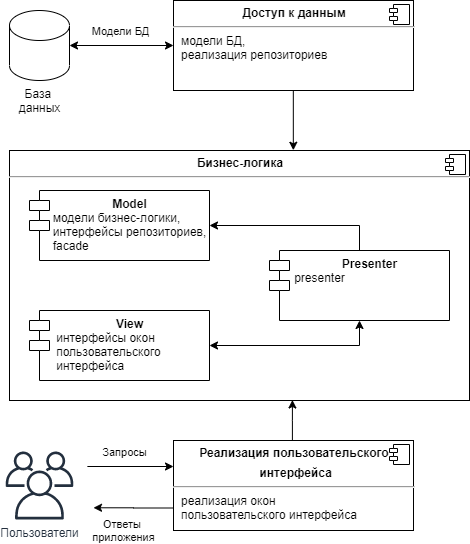
\includegraphics[scale=0.6]{../imgs/uml/components.png}
	\end{center}
	\captionsetup{justification=centering}
	\caption{Архитектура приложения}
	\label{img:components}
\end{figure}

Компонент бизнес-логики спроектирован по схеме MVP (Model-View-Presenter) и является главным (независимым). Он отвечает за логику обработки запросов и данных.

Компонент доступа к данным отвечает за получение данных из БД, их изменение, добавление и удаление. Для его реализации использован паттерн <<репозиторий>>. 

Компонент реализации пользовательского интерфейса предоставляет реализацию UI для выбранного технологического стека.


\section{Выбор in-memory СУБД}


Система управления базами данных (СУБД) -- это совокупность программных и лингвистических средств общего или специального назначения, обеспечивающих управление созданием и использованием баз данных\cite{database}.

В пункте \ref{imdb} среди подходов к хранению данных был сделан выбор в пользу IMDB-систем, поэтому далее будет приведен обзор in-memory СУБД и произведен выбор наиболее подходящей для поставленной задачи.




\subsection{Memcached}

Memcached - это высокопроизводительная система кэширования данных в оперативной памяти, предназначенная для использования в ускорении динамических веб-приложений за счет уменьшения нагрузки на базу данных. Memcached относится к семейству решений для управления данными NoSQL и основана на модели данных с ключевыми значениями  \cite{memcash}. 

Данная СУБД спроектирована так, чтобы все операции имели алгоритмическую сложность O(1), то есть время выполнения любой операции не зависит от количества хранящихся ключей. Это означает, что некоторые операции или возможности, реализация которых требует всего лишь линейного (O(n)) времени, в ней отсутствуют. Так, например, в Memcached отсутствует возможность группировки ключей.


Memcached не является надежным хранилищем – возможна ситуация, когда ключ будет удален из кэша раньше окончания его срока жизни. 

Управление внутренней памятью Memcached более эффективно в простейших случаях использования (при кэшировании относительно небольших и статических данных), поскольку оно потребляет сравнительно мало ресурсов памяти для метаданных. Строки (единственный тип данных, поддерживаемый Memcached) идеально подходят для хранения данных, которые только читаются, потому что строки не требуют дальнейшей обработки. Тем не менее, эффективность управления памятью Memcached быстро уменьшается, когда размер данных является динамическим, после чего память Memcached может стать фрагментированной \cite{memcash2}. 

Еще одно преимущество Memcached -- достаточно простая масштабируемость: поскольку данная система многопоточна, ее можно увеличить, просто предоставив больше вычислительных ресурсов. Однако это может привести к потере части или всех кэшированных данных (в зависимости от того, используется ли постоянное хеширование). 

\subsection{Redis}


Redis \cite{redis} -- резидентная система управлениями базами данных класса NoSQL с открытым исходным кодом. 

Основной структурой данных, с которой работает Redis является структура типа <<ключ-значение>>, причем значения могут быть пяти различных типов. Данная СУБД используется как для хранения данных, так и для реализации кэшей и брокеров сообщений.

Redis хранит данные в оперативной памяти и снабжена механизмом <<снимков>> и журналирования, что обеспечивает постоянное хранение данных. Существует поддержка репликации данных типа master-slave, транзакций и пакетной обработки комманд.

Redis позволяет осуществлять мелкомасштабный контроль за вытеснением данных, предоставляя выбор из шести различных политик вытеснения \cite{redis2}. 

К недостаткам Redis можно отнести отсутствие вторичных индексов и триггеров. Также транзакции в данной СУБД не удовлетворяют свойствам ACID (Atomicity -- Атомарность, Consistency -- Согласованность, Isolation -- Изолированность, Durability -- Долговечность) \cite{acid}.


\subsection{Tarantool}


Tarantool \cite{tarantool} -- это платформа in-memory вычислений с гибкой схемой хранения данных для эффективного создания высоконагруженных приложений. Включает себя базу данных и сервер приложений на языке программирования Lua \cite{lua}.

Записи в Tarantool хранятся в пространствах (space) -- аналог таблицы в реляционной базе данных SQL. Внутри пространства находятся кортежи (tuples), которые похожи на строку в таблице SQL. 


Tarantool объединяет в себе преимущества, характерные для кэша:
\begin{itemize}
	\item <<горячие данные>>;
	\item оптимальная работа при высокой параллельной нагрузке;
	\item низкая задержка (99\% запросов < 1 мс, 99,9\% запросов < 3 мс);
	\item поддерживаемая загрузка на запись — до 1 миллиона транзакций в секунду на одном ядре ЦПУ;
	\item система работает постоянно, не нужно делать перерыв на профилактические работы,
\end{itemize}
и достоинства классических СУБД:
\begin{itemize}
	\item персистентность;
	\item транзакции со свойствами ACID;
	\item наличие репликации (master-slave и master-master);
	\item наличие хранимых процедуры.
	\item поддержка первичных и вторичных индексов (в том числе, составных).
\end{itemize}


В Tarantool реализован механизм <<снимков>> текущего состояния хранилища и журналирования всех операций, что позволяет восстановить состояние базы данных после ее перезагрузки.

К недостаткам данной СУБД можно отнести относительно малое количество поддерживаемых языков (C, C\#, C++, Erlang, Go, Java, JavaScript, Lua, Perl, PHP, Python, Rust) \cite{tarantool}, а также более высокий порог входа по сравнению с ранее рассмотренными СУБД \cite{redis2}.


\subsection{Выбор СУБД для решения задачи}

В данной работе не предполагается хранение в БД очень большого количества информации, и в этом случае требованию о коротком времени отклика удовлетворяют все рассмотренные СУБД.

Рассмотрим несколько требований, которым должна удовлетворять СУБД для решения поставленной задачи.

\begin{enumerate}
	\item Для удобного хранения данных, указанных в пункте \ref{data}, СУБД должна предоставлять, как минимум , два типа данных -- строки и целые числа. 
	\item Для предоставления пользователям перечисленных в пункте \ref{functions} функций, в СУБД должна быть реализована возможность создания вторичных индексов, а также триггеров или хранимых процедур для выполнения сложных вычислений. 
	\item Необходимо надежное хранение данных, без риска их потери даже в случае сбоя в системе (то есть поддержка репликации данных).
\end{enumerate} 


В таблице \ref{tbl:imdb} приведено сравнение рассмотренных СУБД по перечисленным критериям.

\captionsetup{justification=raggedleft,singlelinecheck=off}
\begin{table}[H]
	\centering
	\caption{Сравнение in-memory СУБД}
	\label{tbl:imdb}
	\begin{tabular}{|l|l|l|l|} 
	\hline
	Название  & Требование 1 & Требование 2 & Требование 3  \\ 
	\hline
	Memcached & -            & -            & -             \\ 
	\hline
	Redis     & +            & -            & +             \\ 
	\hline
	Tarantool & +            & +            & +             \\
	\hline
\end{tabular}
\end{table}


Из рассмотренных in-memory СУБД всем перечисленным требованиям удовлетворяет Tarantool, поэтому именно он был выбран для использования в данной работе.




\section{Выбор инструментов разработки}

В качестве языка программирования выбран язык C\# \cite{sharp}. Во-первых, он объектно-ориентирован, что позволит использовать наследование, интерфейсы, абстракции и так далее. Во-вторых, C\# имеет коннектор \\progaudi.tarantool \cite{connector} для платформы in-memory вычислений Tarantool.


В качестве среды разработки была выбрана <<Microsoft Visual Studio 2022>> \cite{vs}, поскольку она:
\begin{itemize}
	\item[1)] имеет множество удобств для написания и отладки кода;
	\item[2)] является бесплатной для студентов;
	\item[3)] обеспечивает работу с фреймворком Windows Forms\cite{wf}, который был выбран для реализации пользовательского интерфейса из-за своей простоты в реализации.  
\end{itemize}

Для упаковки приложения в готовый продукт была выбрана система контейнеризации Docker \cite{docker}. С его помощью можно создать изолированную среду для программного обеспечения, которое можно будет развернуть на различных устройствах без дополнительных настроек.

Тестирование программного продукта производилось с помощью фреймворка xUnit \cite{test}. Данный фреймворк позволяет писать функциональные тесты. 

\section{Детали реализации}

\subsection{Ролевая модель}

Необходимо реализовать ролевую модель в соответствии с пунктом \ref{functions}. Роль – это разрешение, предоставляемое группе пользователей для доступа к данным. 

Ролевая модель реализована на нескольких уровнях, в том числе, на уровне базы данных, что продемонстрировано в листинге \ref{lst:role1}. Последовательно создаются и наделяются правами роли неавторизованного пользователя, авторизованного пользователя, сотрудника лыжного патруля и администратора, каждый наследует и расширяет права предыдущего.

\captionsetup{justification=centering,singlelinecheck=off}
\begin{lstlisting}[label=lst:role1, caption=Ролевая модель на уровне БД, style=myLuastyle]
box.schema.role.create('unauthorized_user')
box.schema.role.grant('unauthorized_user', 'read', 'space', 'lifts', {if_not_exists=true})
box.schema.role.grant('unauthorized_user', 'read', 'space', 'slopes', {if_not_exists=true})
box.schema.role.grant('unauthorized_user', 'read', 'space', 'lifts_slopes', {if_not_exists=true})


box.schema.role.create('authorized_user')
box.schema.role.grant('authorized_user', 'unauthorized_user')
box.schema.role.grant('authorized_user', 'read,write', 'space', 'messages', {if_not_exists=true})

box.schema.role.create('ski_patrol')
box.schema.role.grant('ski_patrol', 'authorized_user')
box.schema.role.grant('unauthorized_user', 'write', 'space', 'lifts', {if_not_exists=true})
box.schema.role.grant('unauthorized_user', 'write', 'space', 'slopes', {if_not_exists=true})
box.schema.role.grant('unauthorized_user', 'write', 'space', 'lifts_slopes', {if_not_exists=true})

box.schema.role.create('ski_admin')
box.schema.role.grant('ski_admin', 'read,write,execute,create,alter,drop', 'universe')
\end{lstlisting}

\subsection{Реализация функции для расчета времени в очереди на подъемник}

В листинге \ref{lst:func} представлены реализации функций update\_queue\_time и count\_card\_readings, предназначенных для обновленияя время в очереди к подъемнику. Алгоритм работы этих функций был описан в пункте \ref{func_label}.


\captionsetup{justification=centering,singlelinecheck=off}
\begin{lstlisting}[label=lst:func, caption=Функции update\_queue\_time и count\_card\_readings, style=myLuastyle]
function count_card_readings(lift_id, date_from, date_query)
	connected_turnstiles = turnstiles.index.index_lift_id:select({lift_id})
	counter = 0
	for k,v in pairs(connected_turnstiles) do
		cur_turnstile_id = v["turnstile_id"]
		card_readings_on_turnstile = card_readings.index.index_turnstile:select({cur_turnstile_id})
		
		for k,v in pairs(card_readings_on_turnstile) do
			if (v["reading_time"] >= date_from and v["reading_time"] < date_query) then
				counter = counter + 1
			end
		end
	end
	return counter
end
function update_queue_time(lift_id, date_from, date_query)
	card_readings_amount = count_card_readings(lift_id, date_from, date_query)
	lift = lifts:get{lift_id}
	time_delta = date_query - date_from
	new_queue_time = math_module.max(math_module.ceil(
			lift["queue_time"] - time_delta  + 
			(card_readings_amount * lift["lifting_time"] * 2 / lift["seats_amount"])), 0)
	lifts:update(lift_id, {{'=', 6, new_queue_time}})
	return new_queue_time
end
\end{lstlisting}

\subsection{Модели хранения данных}

На примере таблицы спусков slopes рассмотрим модель хранения данных и реализацию доступа к данным.

В листинге \ref{lst:slopes_tarantool} продемонстрировано создание спейса (таблицы) slopes в БД. Особенность Tarantool заключается в том, что для поиска кортежа (строки) в спейсе по значению его поля, это поле должно быть проиндексировано. Так как в спейсе slopes будет необходимо искать кортежи как по значению поля slope\_id (PK), так и по значению поля slope\_name, то для этого спейса необходимо создать два соответствующих индекса (первичный и вторичный).

\captionsetup{justification=centering,singlelinecheck=off}
\begin{lstlisting}[label=lst:slopes_tarantool, caption=Создание спейса slopes, style=myLuastyle]
slopes = box.schema.space.create('slopes', {field_count=4})
slopes:format({
	{name = 'slope_id', type = 'unsigned'},
	{name = 'slope_name', type = 'string'},
	{name = 'is_open', type = 'boolean'},
	{name = 'difficulty_level', type = 'unsigned'}})
slopes:create_index('primary')
slopes:create_index('index_name', {parts = {'slope_name'}})
\end{lstlisting}

В листинге \ref{lst:slopes_bl} приведена реализация модели slopes, используемой в компоненте бизнес-логики. Отношение между таблицами slopes и lifts многие-ко-многим здесь реализована с помощью хранения связанных со спуском подъемников в модели спусков, и наоборот. Связанные объекты добавляются в модель по запросу.

\captionsetup{justification=centering,singlelinecheck=off}
\begin{lstlisting}[label=lst:slopes_bl, caption=Модель базы данных на примере таблицы slopes, language=csharp]
public record class Slope {
	public uint SlopeID { get; }
	public string SlopeName { get;}
	public bool IsOpen { get; }
	public uint DifficultyLevel { get; }
	public List<Lift>? ConnectedLifts { get; }

	public Slope(uint slopeID, string slopeName, bool isOpen, uint difficultyLevel){
		this.SlopeID = slopeID;
		this.SlopeName = slopeName;
		this.IsOpen = isOpen;
		this.DifficultyLevel = difficultyLevel;}
	public Slope(Slope slope, List<Lift> connectedLifts){
		this.SlopeID = slope.SlopeID;
		this.SlopeName = slope.SlopeName;
		this.IsOpen = slope.IsOpen;
		this.DifficultyLevel = slope.DifficultyLevel;
		this.ConnectedLifts = connectedLifts;}
}
\end{lstlisting}

В листинге \ref{lst:slopes_rep} приведена часть реализации репозитория \\TarantoolSlopesRepository, который обеспечивает доступ к данным спейса slopes из БД. Отражены функция GetSlopeByNameAsync, осуществляющая поиск спуска по его названию с помощью ранее созданного вторичного индекса, а также функция AddSlopeAutoIncrementAsync, которая осуществляет вставку нового кортежа, используя первичный ключ с автоматическим увеличением.

\captionsetup{justification=centering,singlelinecheck=off}
\begin{lstlisting}[label=lst:slopes_rep, caption=Часть реализации репозитория для доступа к данным спейса slopes из БД, language=csharp]
public class TarantoolSlopesRepository : ISlopesRepository
{
	private IIndex _indexPrimary;
	private IIndex _indexName;
	private ISpace _space;
	private IBox _box;
	...
	
	public async Task<Slope> GetSlopeByNameAsync(string name)
	{
		var data = await _indexName.Select<ValueTuple<string>, SlopeDB>
		(ValueTuple.Create(name));
		
		if (data.Data.Length != 1)
		{
			throw new SlopeNotFoundException($"Error: couldn't find slope with name={name}");
		}
		
		return SlopeConverter.DBToBL(data.Data[0]);
	}
	
	public async Task<uint> AddSlopeAutoIncrementAsync(string slopeName, bool isOpen, uint difficultyLevel)
	{
		try
		{
			var result = await _box.Call_1_6<SlopeDBNoIndex, SlopeDB>("auto_increment_slopes", (new SlopeDBNoIndex(slopeName, isOpen, difficultyLevel)));
			return SlopeConverter.DBToBL(result.Data[0]).SlopeID;
		}
		catch (Exception ex)
		{
			throw new SlopeAddAutoIncrementException();
		}
	}
	...
}
\end{lstlisting}

В используемом коннекторе progaudi.tarantool не реализована соответствующая функция <<space\_object:auto\_increment()>> СУБД Tarantool, поэтому на уровне базы данных для каждого спейса реализованы обертки для данной функции и конкретного спейса. Именно они вызываются из приложения, что продемонстрировано в функции AddSlopeAutoIncrementAsync в листинге выше. Пример такой функции-обертки на уровне БД приведен в листинге \ref{lst:ob}.

\captionsetup{justification=centering,singlelinecheck=off}
\begin{lstlisting}[label=lst:ob, caption=Обертка для функции <<space\_object:auto\_increment()>> и спейса slopes, style=myLuastyle]
function auto_increment_slopes(slope_name, is_open, difficulty_level)
	return box.space.slopes:auto_increment{slope_name, is_open, difficulty_level}
end

\end{lstlisting}

\section{Интерфейс приложения}


При запуске приложения пользователь считается неавторизованным. Открывается главное окно, продемонстрированное на рисунке \ref{img:main}, в котором размещены кнопки для открытия других окон. 

\clearpage
\begin{figure}[h!]
	\begin{center}
		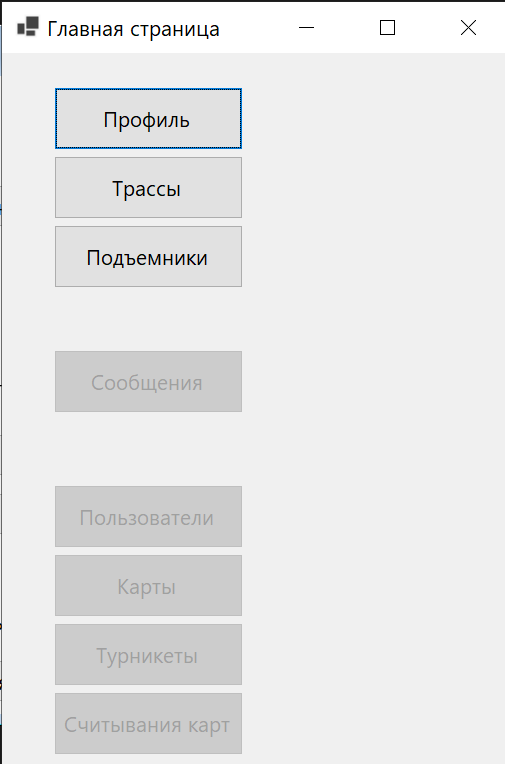
\includegraphics[scale=0.8]{../imgs/int/main.png}
	\end{center}
	\captionsetup{justification=centering}
	\caption{Главное окно приложения (пользователь не авторизован)}
	\label{img:main}
\end{figure}

В любом окне неактивная кнопка означает, что данное действие недоступно данному пользователю. Например, в окне <<Профиль>> неавторизованный пользователь может только выполнить вход или зарегистрироваться (рисунок \ref{img:profu}), авторизованный -- только выполнить выход (рисунок \ref{img:profa}).


\begin{figure}[h!]
	\begin{center}
		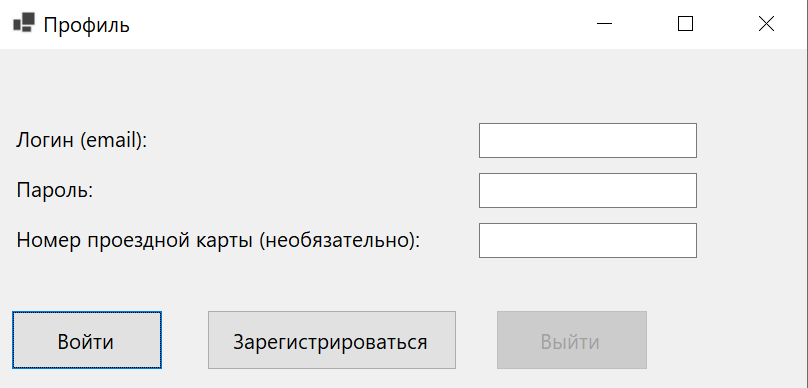
\includegraphics[scale=1]{../imgs/int/profu.png}
	\end{center}
	\captionsetup{justification=centering}
	\caption{Окно <<Профиль>> (пользователь не авторизован)}
	\label{img:profu}
\end{figure}

\clearpage
\begin{figure}[h!]
	\begin{center}
		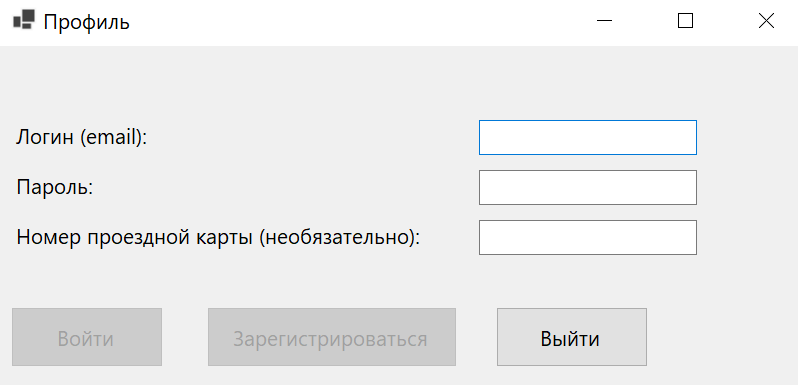
\includegraphics[scale=1]{../imgs/int/profa.png}
	\end{center}
	\captionsetup{justification=centering}
	\caption{Окно <<Профиль>> (пользователь авторизован)}
	\label{img:profa}
\end{figure}

Далее для демонстрации всех функций системы окна будут показаны в том виде, в котором они открываются для пользователя с правами администратора, так как ему доступен наибольший функционал.

На рисунке \ref{img:messages} показан вид окна <<Сообщения>>. Предоставляется возможность получить информацию обо всех сообщениях или об одном из них по ID; добавить (отправить), изменить (в частности, отметить прочитанным) или удалить сообщение.

%\clearpage
\begin{figure}[h!]
	\begin{center}
		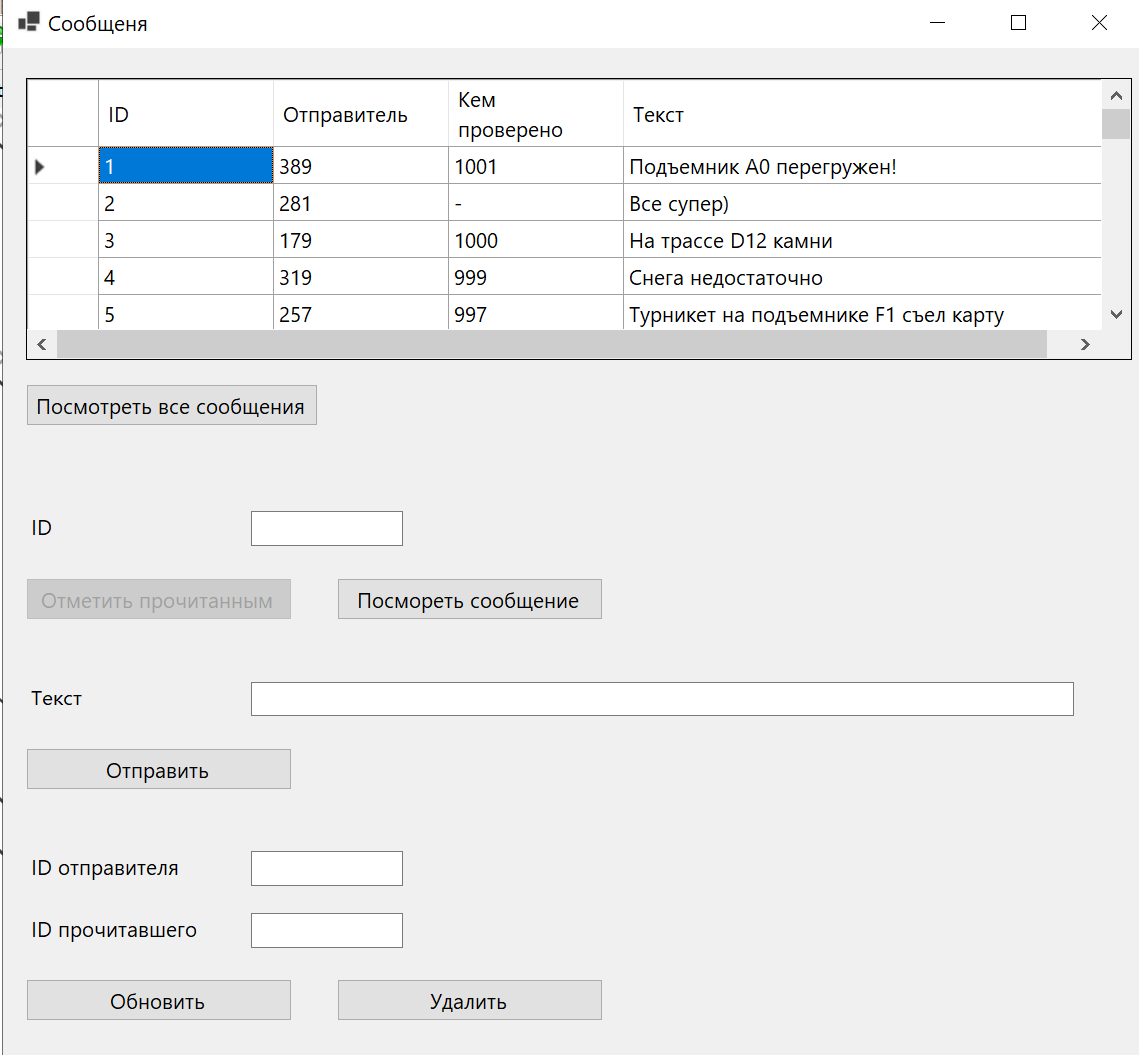
\includegraphics[scale=0.65]{../imgs/int/messages.png}
	\end{center}
	\captionsetup{justification=centering}
	\caption{Окно <<Сообщения>>}
	\label{img:messages}
\end{figure}


На рисунке \ref{img:slopes} показан вид окна <<Трассы>>. Предоставляется возможность получить информацию обо всех трассах или об одной из них по названию; добавить, изменить или удалить трассу; добавить или удалить связь с подъемником.


\begin{figure}[h!]
	\begin{center}
		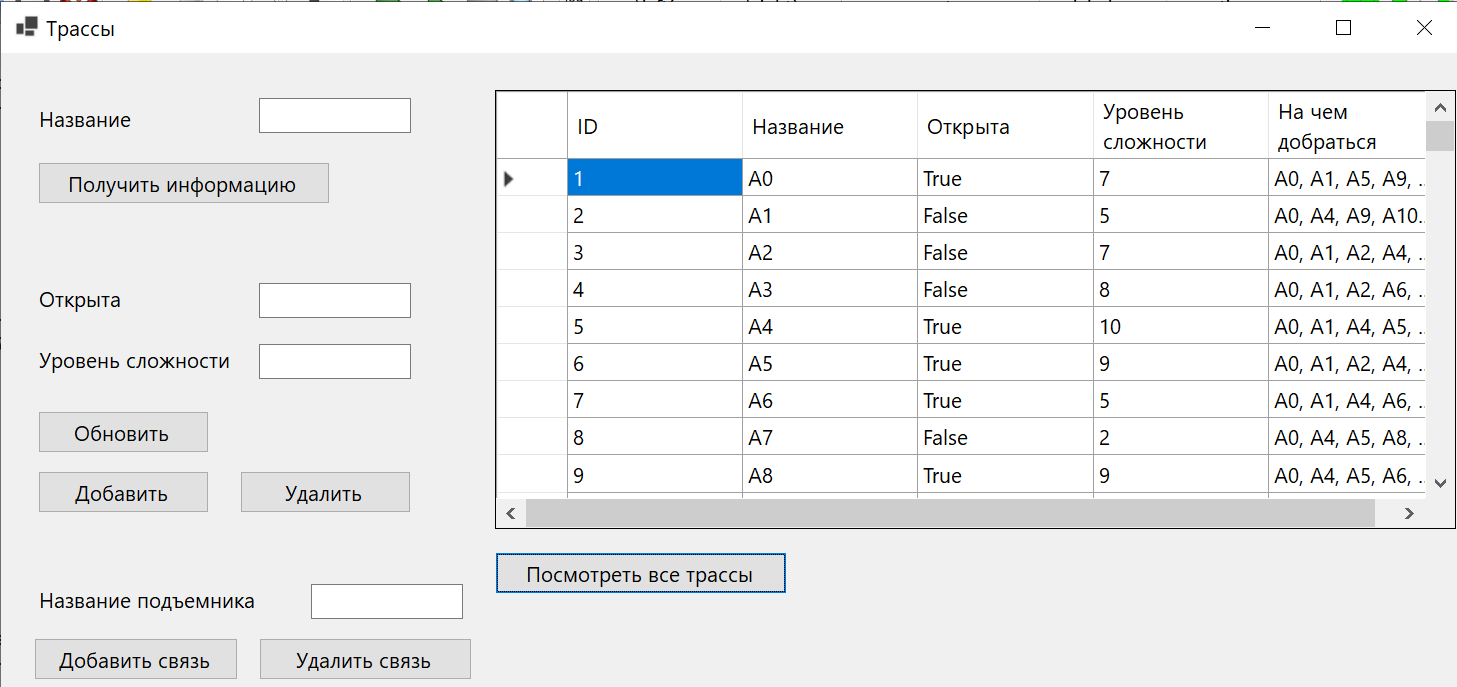
\includegraphics[scale=0.7]{../imgs/int/slopes.png}
	\end{center}
	\captionsetup{justification=centering}
	\caption{Окно <<Трассы>>}
	\label{img:slopes}
\end{figure}

На рисунке \ref{img:lifts} показан вид окна <<Подъемники>>. Предоставляется возможность получить информацию обо всех подъемниках или об одном из них по названию; добавить, изменить или удалить подъемник; добавить или удалить связь с трассой.

\clearpage
\begin{figure}[h!]
	\begin{center}
		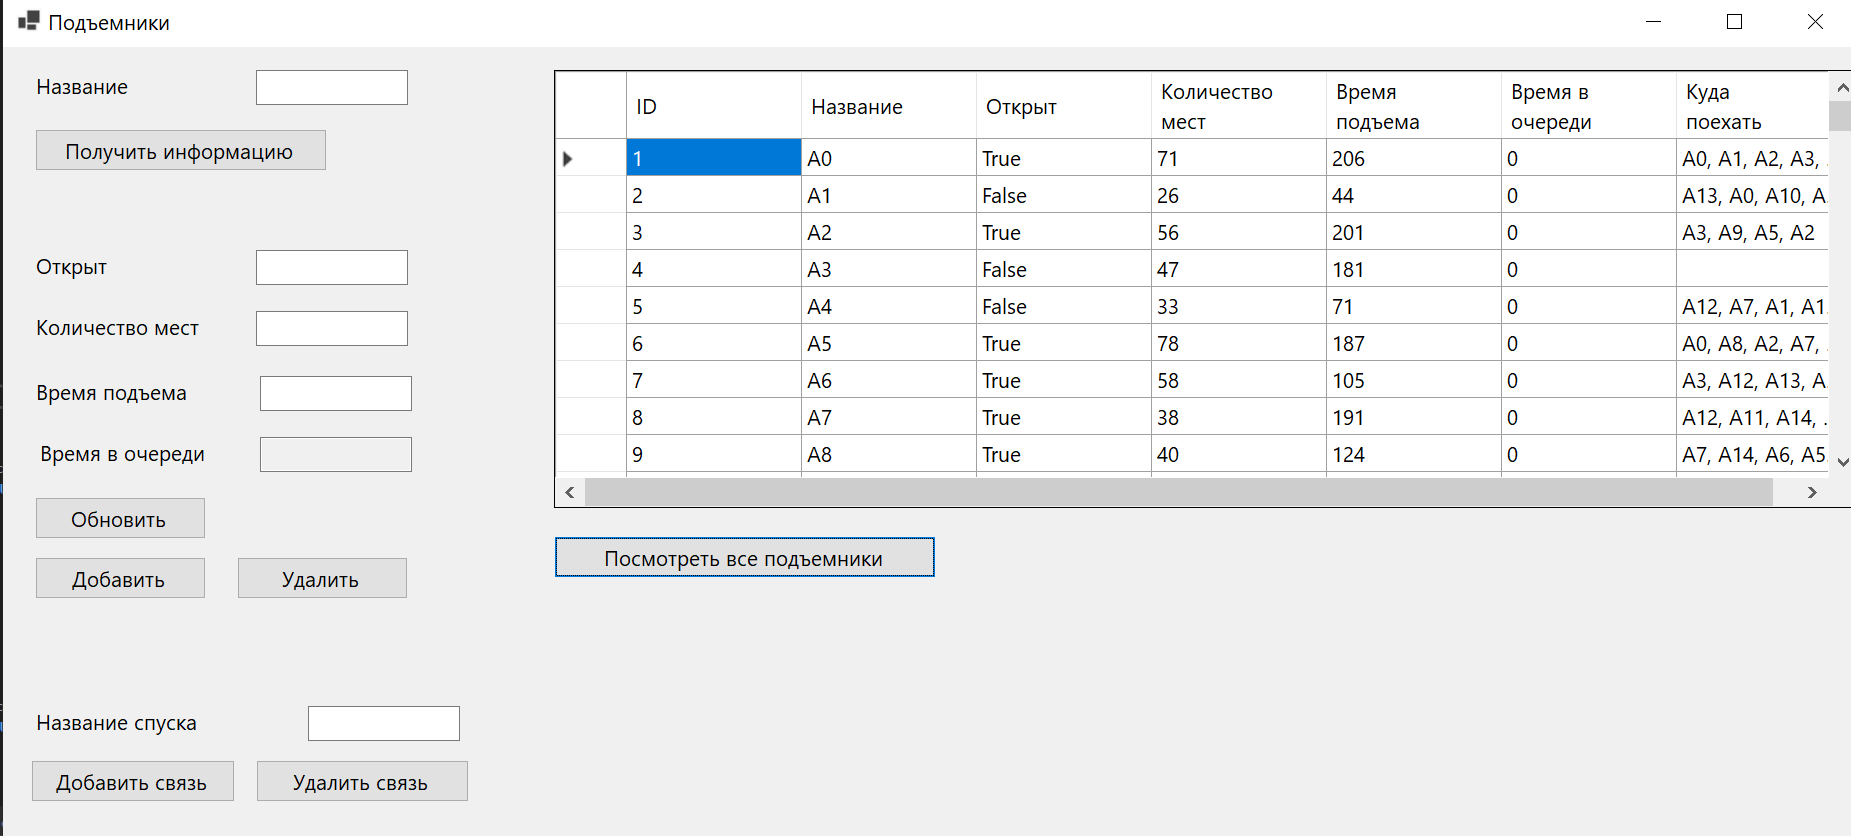
\includegraphics[scale=0.55]{../imgs/int/lifts.png}
	\end{center}
	\captionsetup{justification=centering}
	\caption{Окно <<Подъемники>>}
	\label{img:lifts}
\end{figure}

На рисунках \ref{img:users}, \ref{img:cards}, \ref{img:turnstiles}, \ref{img:readings} показаны виды окон <<Пользователи>>, <<Карты>>, <<Турникеты>> и <<Считывания карт>>, соответственно. В каждом окне можно получить информацию обо всех соответствующих объектах или об одном из них по ID; добавить, изменить или удалить объект.

\begin{figure}[h!]
	\begin{center}
		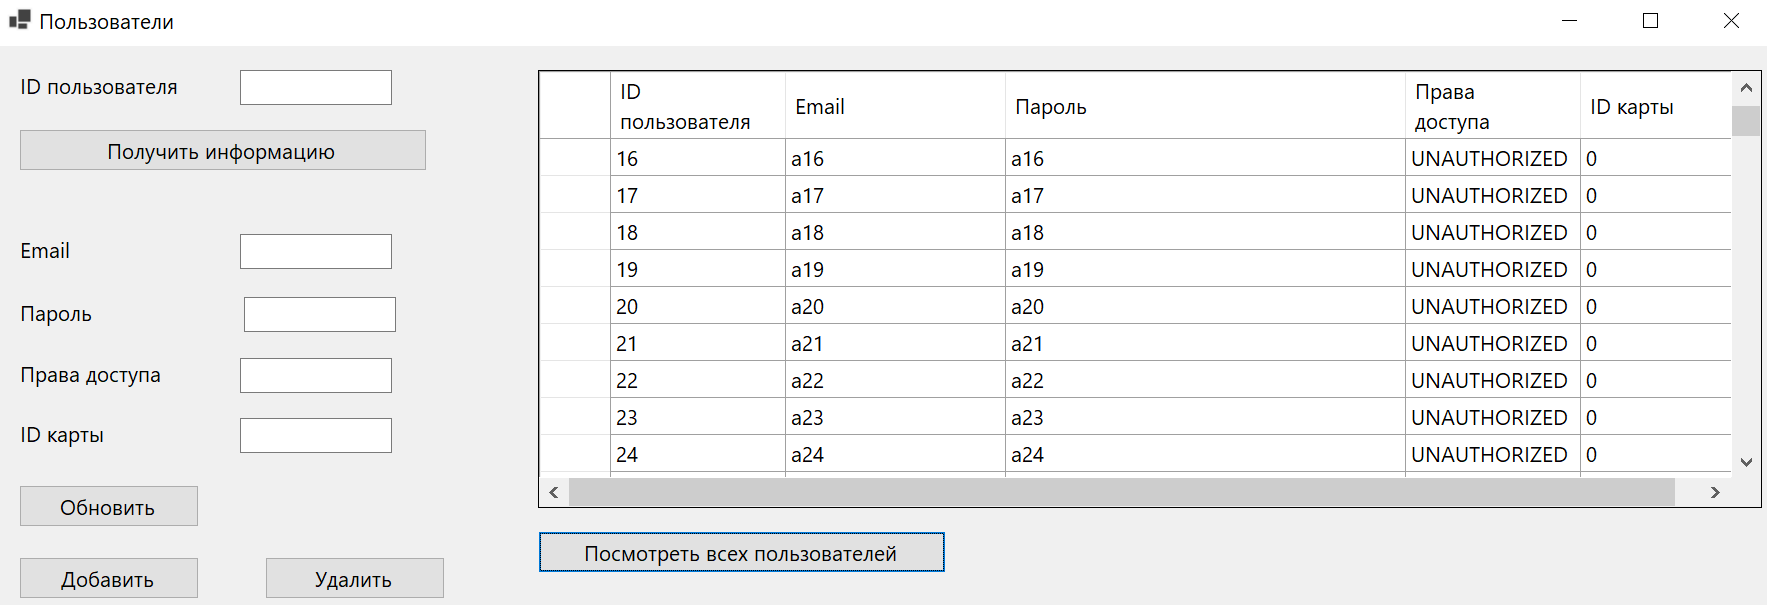
\includegraphics[scale=0.6]{../imgs/int/users.png}
	\end{center}
	\captionsetup{justification=centering}
	\caption{Окно <<Пользователи>>}
	\label{img:users}
\end{figure}

\begin{figure}[h!]
	\begin{center}
		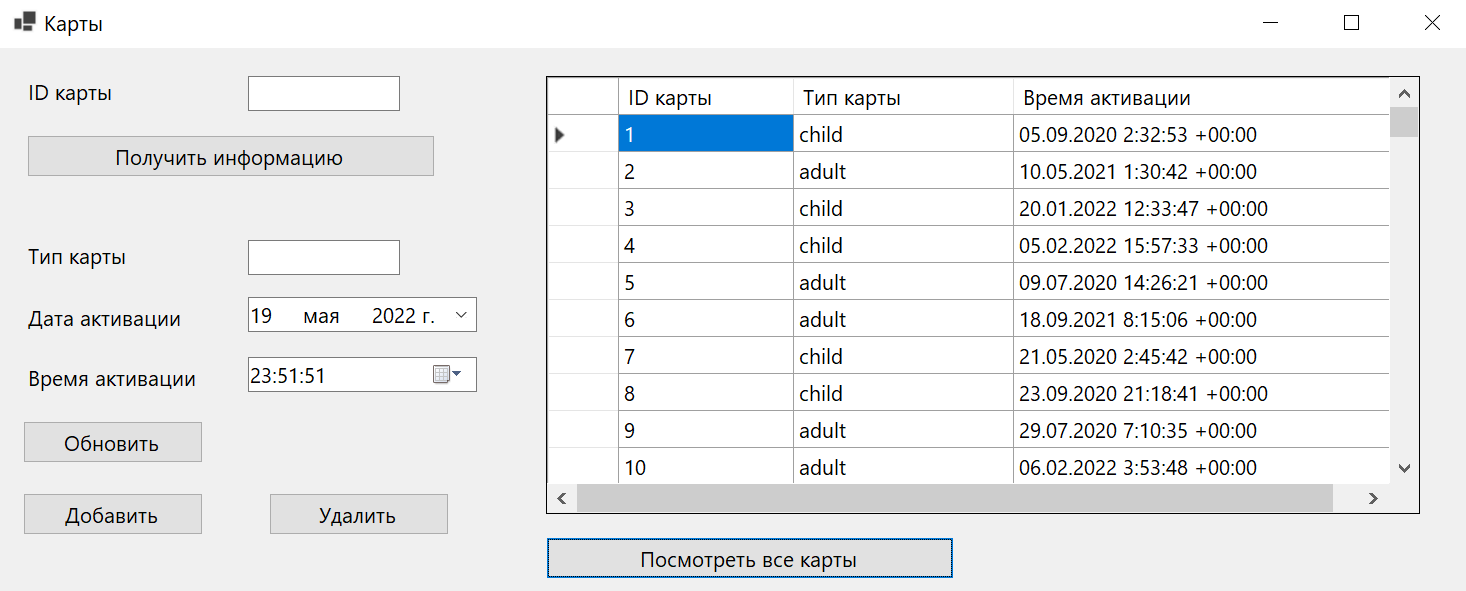
\includegraphics[scale=0.6]{../imgs/int/cards.png}
	\end{center}
	\captionsetup{justification=centering}
	\caption{Окно <<Карты>>}
	\label{img:cards}
\end{figure}

\begin{figure}[h!]
	\begin{center}
		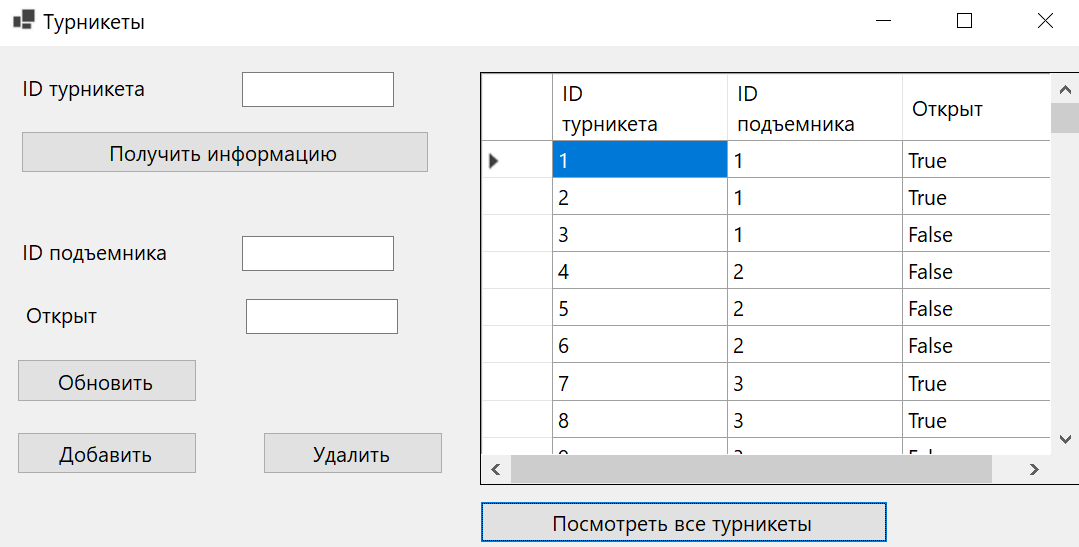
\includegraphics[scale=0.6]{../imgs/int/turnstiles.png}
	\end{center}
	\captionsetup{justification=centering}
	\caption{Окно <<Турникеты>>}
	\label{img:turnstiles}
\end{figure}

\begin{figure}[h!]
	\begin{center}
		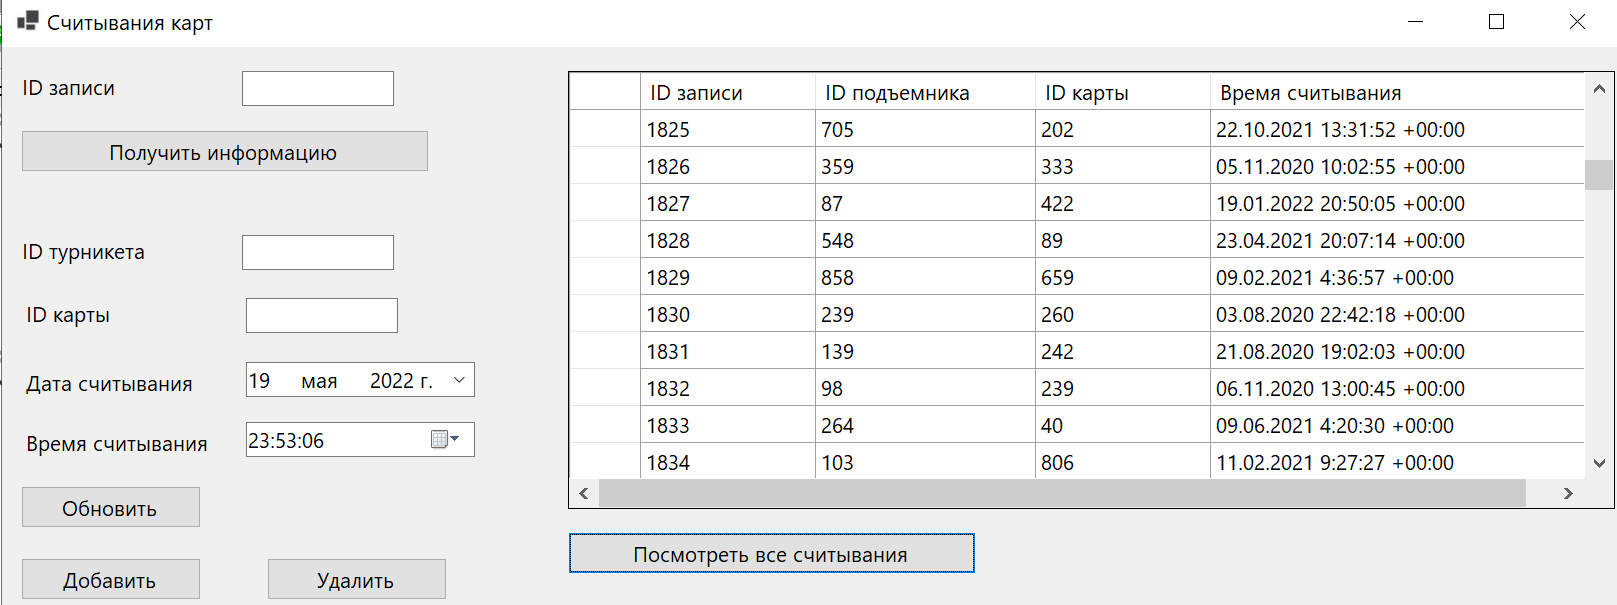
\includegraphics[scale=0.6]{../imgs/int/readings.png}
	\end{center}
	\captionsetup{justification=centering}
	\caption{Окно <<Считывания карт>>}
	\label{img:readings}
\end{figure}

\clearpage
\section*{Вывод}

На основе анализа in-memory СУБД был осуществлен выбор наиболее подходящей для решения поставленной задачи. Была спроектирована архитектура приложения, выбраны инструменты разработки, приведены детали реализации и интерфейс приложения.